\documentclass[12pt, oneside]{article}
\usepackage[letterpaper, margin=1in, headsep=0.5in, left=0.3in, right=2.5in]{geometry}
\usepackage[english]{babel}
\usepackage[utf8]{inputenc}
\usepackage{amsmath}
\usepackage{amsfonts}
\usepackage{amssymb}
\usepackage{tikz}
\usepackage{yhmath}
\usetikzlibrary{quotes, angles}
\usepackage{graphicx}
\usepackage{enumitem}
\usepackage{multicol}

\newif\ifmeta
\metatrue %print standards and topics tags

\title{Regents Geometry}
\author{Chris Huson}
\date{April 2022}

\usepackage{fancyhdr}
\pagestyle{fancy}
\fancyhf{}
\renewcommand{\headrulewidth}{0pt} % disable the underline of the header
\raggedbottom

%\fancyhead[LE]{\thepage}
\fancyhead[RO]{Name:}
\fancyhead[LO]{BECA / Dr. Huson / Geometry Regents  Advanced Material}
\cfoot{\thepage}

\begin{document}
\subsubsection*{11.3 Regents: Similar triangles in circles \hfill GEO-G.C.2b}
\begin{enumerate}[itemsep=1.7cm]
\item As shown, circle $O$ has chords $\overline{AD}$ and $\overline{BE}$ intersecting at $C$, and $m \wideparen{AB}=70^\circ$, $m \wideparen{BD}=80^\circ$, $m \wideparen{AE}=100^\circ$, and $m \wideparen{DE}=110^\circ$. $BC=3$, $AC=4$, and $CE=6$.
  \begin{multicols}{2}
  \raggedcolumns
  \begin{flushright}
    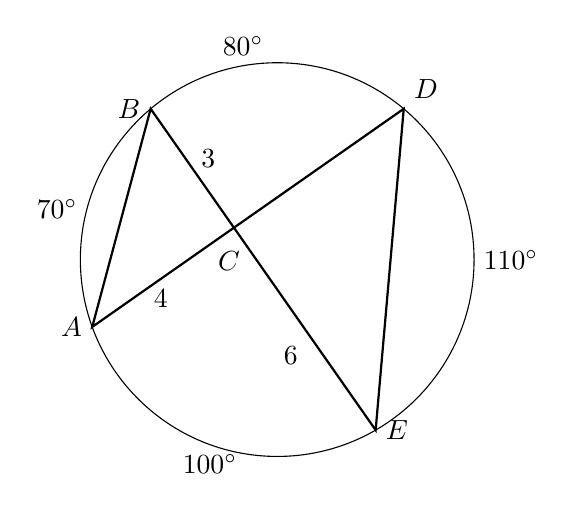
\begin{tikzpicture}[scale=.5]
    \draw (0,0) circle[radius=5];
    \draw [thick]
    (-60:5) node[right] {$E$}--
    (130:5) node[left] {$B$}--
    (200:5) node[left] {$A$}--
    (50:5) node[above right] {$D$}--cycle;
    \draw (160:1.3) node[below] {$C$};
    \draw (120:3.5) node[below] {$3$};
    \draw (190:3) node[below] {$4$};
    \draw (280:2.0) node[below] {$6$};
    \draw (0:5) node[right] {$110^\circ$};
    \draw (100:5) node[above] {$80^\circ$};
    \draw (165:5) node[left] {$70^\circ$};
    \draw (250:5) node[below] {$100^\circ$};
    \end{tikzpicture}
  \end{flushright}
  \begin{enumerate}
    \item Write down the measure of angles $\angle B$ and $\angle D$. \vspace{0.5cm}
    \item Write down the measure of angles $\angle A$ and $\angle E$. \vspace{0.5cm}
    \item Find the measures of the two angles at $C$. \vspace{1.5cm}
    \item Find the scale factor and $CD$.
    \end{enumerate}
  \end{multicols}
  \vspace{1cm}

\item Given circle $O$ with chords $\overline{AD}$ and $\overline{BE}$ intersecting at $C$, as shown in the diagram. Given $m \wideparen{AB}=45^\circ$, $m \wideparen{BD}=108^\circ$, and $m \wideparen{DE}=65^\circ$.
  \begin{multicols}{2}
  \raggedcolumns
  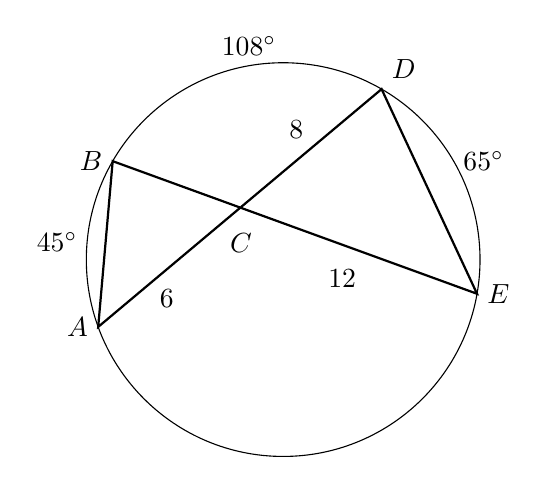
\begin{tikzpicture}[scale=.5]
   \draw (0,0) circle[radius=5];
   \draw [thick]
   (-10:5) node[right] {$E$}--
   (150:5) node[left] {$B$}--
   (200:5) node[left] {$A$}--
   (60:5) node[above right] {$D$}--cycle;
   \draw (140:1.4) node[below] {$C$};
   \draw (30:5) node[right] {$65^\circ$};
   \draw (100:5) node[above] {$108^\circ$};
   \draw (175:5) node[left] {$45^\circ$};
   \draw (85:3.8) node[below] {$8$};
   \draw (190:3) node[below] {$6$};
   \draw (0:1.5) node[below] {$12$};
  \end{tikzpicture}
  \columnbreak
  \begin{enumerate}
    \item Write down the measure of angles $\angle B$ and $\angle D$. \vspace{0.5cm}
    \item Write down the measure of angles $\angle A$ and $\angle E$. \vspace{0.5cm}
    \item Find the measures of the two angles at $C$. \vspace{1.5cm}
    \item Find the scale factor and $BC$.
    \end{enumerate}
  \end{multicols}
  
\newpage
\item The secants $\overline{ABC}$ and $\overline{ADE}$ intersect the circle $O$, as shown in the diagram. \\Given $m \wideparen{BD}=28^\circ$ and $m \wideparen{CE}=136^\circ$.
  \begin{enumerate}
    \item Find the $m\angle CDE$.
    \item Find the $m\angle C$.
    \item Find the $m\angle A$.
  \end{enumerate}
  \begin{center}
  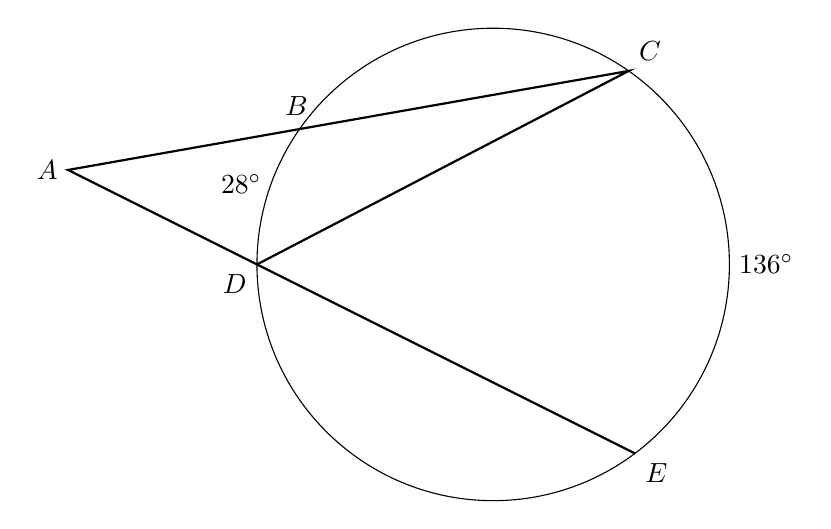
\begin{tikzpicture}[scale=.6]
    \draw (0,0) circle[radius=5];
    \draw [thick]
    (3,-4) node[below right] {$E$}--
    (-5,0) node[below left] {$D$}--
    (-9,2) node[left] {$A$}--
    (55:5) node[above right] {$C$}--
    (-5,0);
    \draw (138:5) node[left] {$B$};
    \draw (0:5) node[right] {$136^\circ$};
    \draw (160:5) node[left] {$28^\circ$};
  \end{tikzpicture}
  \end{center}

\item The secants $\overline{ABC}$ and $\overline{ADE}$ intersect the circle $O$, as shown in the diagram. \\$AB=10$, $AD=8$, $AC=24$. (note: similar triangles)
\begin{multicols}{2}
  \begin{enumerate}
    \item $\overline{AD} \rightarrow \; ?$
    \item $k=$
    \item $\overline{AC} \rightarrow \; ?$
    \item $AE=$
  \end{enumerate}
\end{multicols} \vspace{1cm}
  \begin{center}
  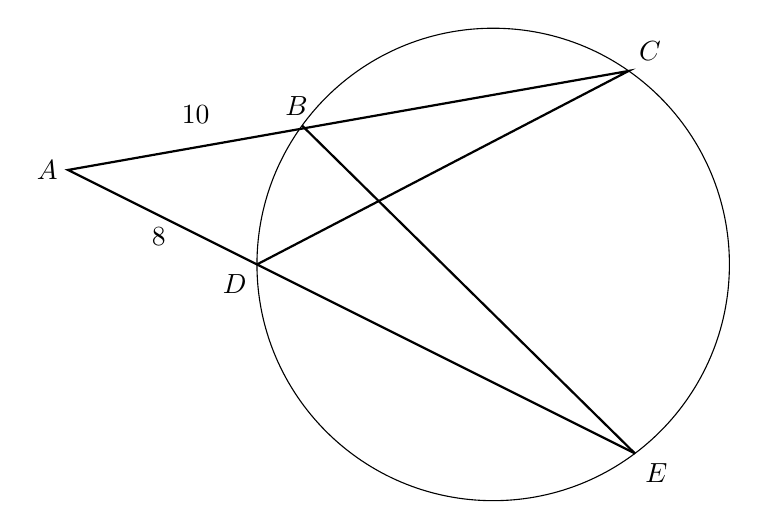
\begin{tikzpicture}[scale=.6]
    \draw (0,0) circle[radius=5];
    \draw [thick]
    (3,-4) node[below right] {$E$}--
    (-5,0) node[below left] {$D$}--
    (-9,2) node[left] {$A$}--
    (55:5) node[above right] {$C$}--
    (-5,0);
    \draw [thick] (3,-4)--(144:5);
    \draw (138:5) node[left] {$B$};
    \draw (155:7.5) node[right] {$10$};
    \draw (175:6.75) node[left] {$8$};
  \end{tikzpicture}
  \end{center}

\newpage
\item Circle $O$ has a radius $AO=8$, as shown below, and $m\angle AOB=60^\circ$.
  \begin{multicols}{2}
    \begin{enumerate}
      \item Find the arc measure $m \wideparen{AB}$. \vspace{1cm}
      \item Find the length of the arc $\wideparen{AB}$. \vspace{1cm}
      \item Find the area of the sector $AOB$. %\vspace{2.5cm}
    \end{enumerate}
    \begin{flushright}
    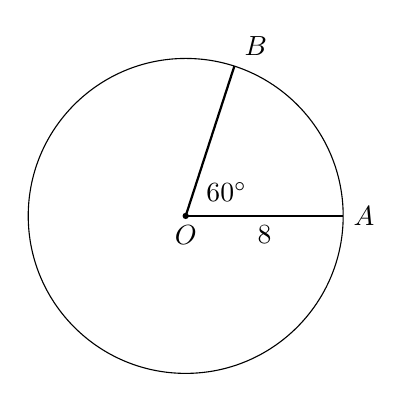
\begin{tikzpicture}[scale=.4]
      \draw (0,0) circle[radius=5];
      \draw [thick]
      (0:5) node[right] {$A$}--(0,0);
      \draw [thick] (0,0)--(72:5) node[above right] {$B$};
      \fill (0,0) circle[radius=0.1] node[below]{$O$};
      \draw (30:1.5) node{$60^\circ$};
      \draw (0:2.5) node[below]{$8$};
    \end{tikzpicture}
  \end{flushright}
  \end{multicols}

\item Given circle $P$ with $m \angle APB=80^\circ$.
\begin{multicols}{2}
\raggedcolumns
\begin{enumerate}
\item Write down the $m \wideparen{AB}$. \vspace{1.7cm}
\item Find the $m\angle AQB$.
\end{enumerate}
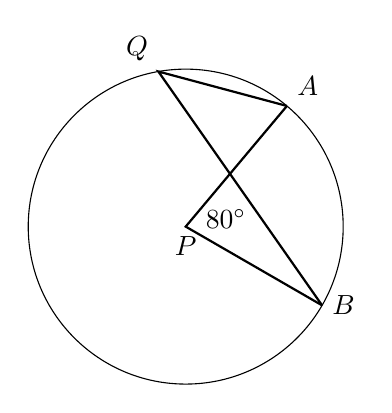
\begin{tikzpicture}[scale=.4]
\draw (0,0) circle[radius=5];
\draw [thick]
(-30:5) node[right] {$B$}--
(0,0) node[below] {$P$}--
(50:5) node[above right] {$A$};
\draw [thick] (-30:5)--(100:5) node[above left] {$Q$}--(50:5);
\draw (35:0.4) node[right]{$80^\circ$};
\end{tikzpicture}
\end{multicols}

\item Given circle $O$ with chords $\overline{AD}$ and $\overline{BE}$ intersecting at $C$, as shown in the diagram. Given $m \wideparen{AB}=40^\circ$, $m \wideparen{BD}=115^\circ$, and $m \wideparen{DE}=70^\circ$.
\begin{multicols}{2}
\raggedcolumns
\begin{enumerate}
\item Find the $m\angle ACB$. \vspace{1.7cm}
\item Find the measure of the minor arc, $m\wideparen{AE}$.
\end{enumerate}
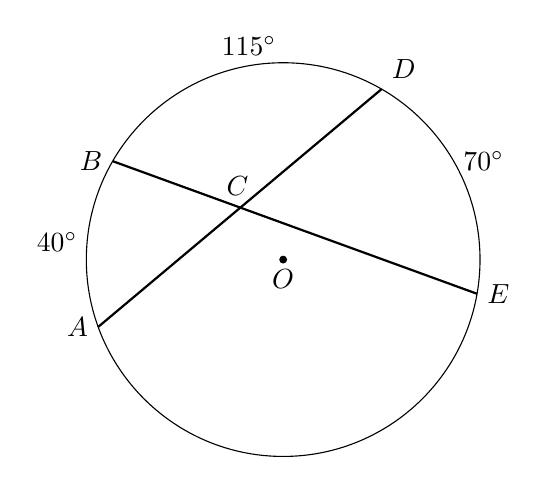
\begin{tikzpicture}[scale=.5]
\draw (0,0) circle[radius=5];
\draw [thick]
(-10:5) node[right] {$E$}--
(150:5) node[left] {$B$};
\draw [thick] (200:5) node[left] {$A$}--
(60:5) node[above right] {$D$};
\draw (130:1.8) node[above] {$C$};
\draw (30:5) node[right] {$70^\circ$};
\draw (100:5) node[above] {$115^\circ$};
\draw (175:5) node[left] {$40^\circ$};
\fill (0,0) circle[radius=0.1] node[below]{$O$};
\end{tikzpicture}
\end{multicols}

\newpage
\item Given circle $O$ with chords $\overline{AD}$ and $\overline{BE}$ intersecting at $C$, as shown in the diagram. Given $m \wideparen{AB}=70^\circ$, $m \wideparen{BD}=80^\circ$, and $m \wideparen{DE}=110^\circ$.
\begin{multicols}{2}
\raggedcolumns
\begin{enumerate}
\item Find the $m\angle BED$. \vspace{1.3cm}
\item Find the $m\angle ACB$. \vspace{2cm}
\item Given $AC=4$ and $BC=3$, find $AB$. \vspace{2cm}
\item Given $CE=6$, find $CD$. \vspace{2cm}
\end{enumerate}
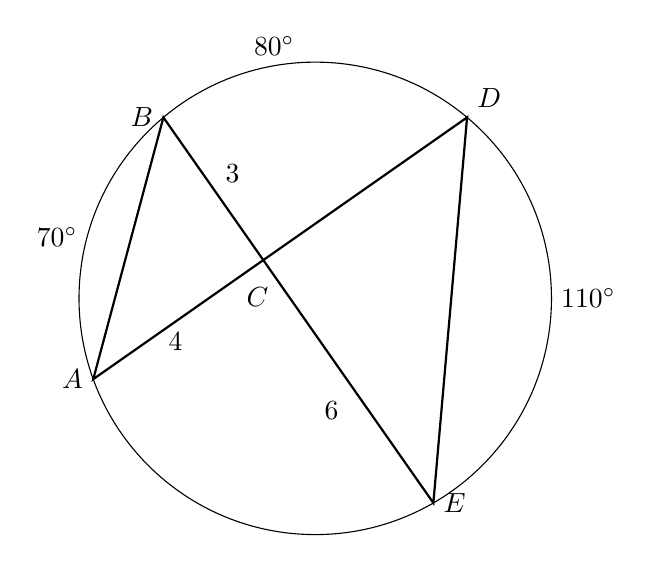
\begin{tikzpicture}[scale=.6]
\draw (0,0) circle[radius=5];
\draw [thick]
(-60:5) node[right] {$E$}--
(130:5) node[left] {$B$}--
(200:5) node[left] {$A$}--
(50:5) node[above right] {$D$}--cycle;
\draw (160:1.3) node[below] {$C$};
\draw (120:3.5) node[below] {$3$};
\draw (190:3) node[below] {$4$};
\draw (280:2.0) node[below] {$6$};
\draw (0:5) node[right] {$110^\circ$};
\draw (100:5) node[above] {$80^\circ$};
\draw (165:5) node[left] {$70^\circ$};
\end{tikzpicture}
\end{multicols}
\vspace{2cm}


\item Given circle $O$ with chords $\overline{AD}$ and $\overline{BE}$ intersecting at $C$, as shown in the diagram. Given $m \wideparen{AB}=45^\circ$, $m \wideparen{BD}=108^\circ$, and $m \wideparen{DE}=65^\circ$.
\begin{multicols}{2}
\raggedcolumns
\begin{enumerate}
 \item Find the $m\angle BAD$. \vspace{1.7cm}
 \item Find the $m\angle ACB$. \vspace{2cm}
\end{enumerate}
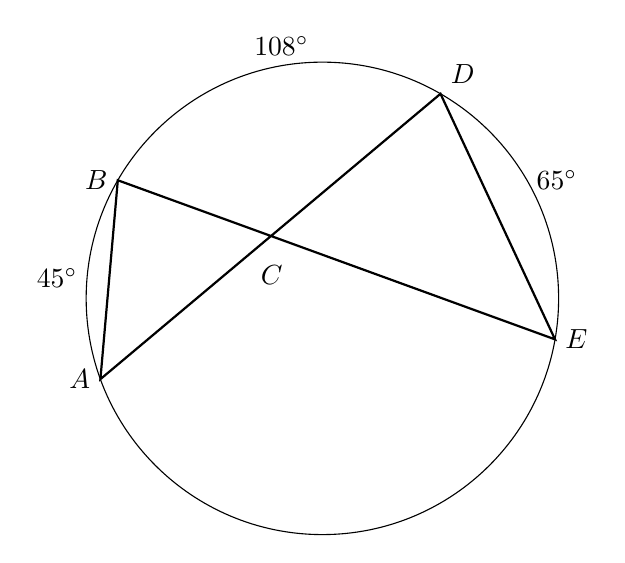
\begin{tikzpicture}[scale=.6]
 \draw (0,0) circle[radius=5];
 \draw [thick]
 (-10:5) node[right] {$E$}--
 (150:5) node[left] {$B$}--
 (200:5) node[left] {$A$}--
 (60:5) node[above right] {$D$}--cycle;
 \draw (140:1.4) node[below] {$C$};
 \draw (30:5) node[right] {$65^\circ$};
 \draw (100:5) node[above] {$108^\circ$};
 \draw (175:5) node[left] {$45^\circ$};
\end{tikzpicture}
\end{multicols}

\newpage

\item The secants $\overline{ABC}$ and $\overline{ADE}$ intersect the circle $O$, as shown in the diagram. \\Given $m \wideparen{BD}=30^\circ$ and $m \wideparen{CE}=140^\circ$. Find the $m\angle A$.
\begin{center}
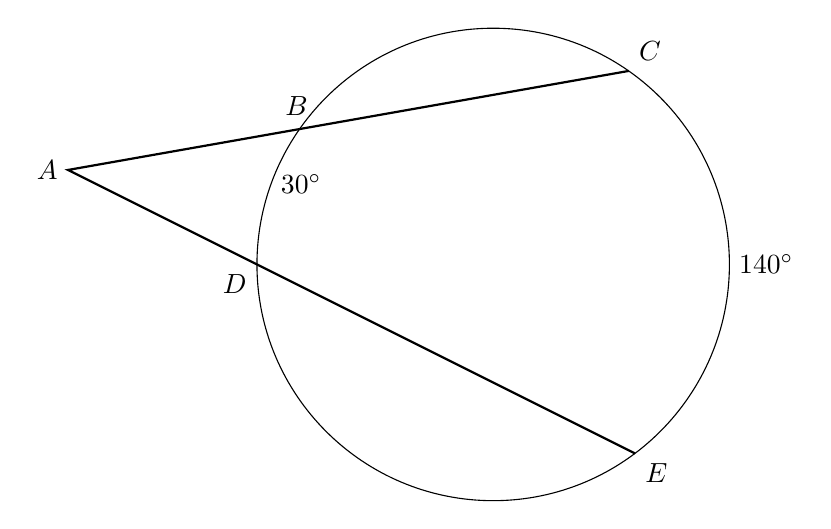
\begin{tikzpicture}[scale=.6]
\draw (0,0) circle[radius=5];
\draw [thick]
(3,-4) node[below right] {$E$}--
(-5,0) node[below left] {$D$}--
(-9,2) node[left] {$A$}--
(55:5) node[above right] {$C$};
\draw (138:5) node[left] {$B$};
\draw (0:5) node[right] {$140^\circ$};
\draw (160:5) node[right] {$30^\circ$};
\end{tikzpicture}
\end{center} \vspace{1cm}

\item The secants $\overline{PQR}$ and $\overline{PST}$ intersect the circle $O$, as shown in the diagram. \\Given $m \angle P=35^\circ$ and $m \wideparen{RT}=120^\circ$. Find the $m\wideparen{QS}$.
  \begin{center}
  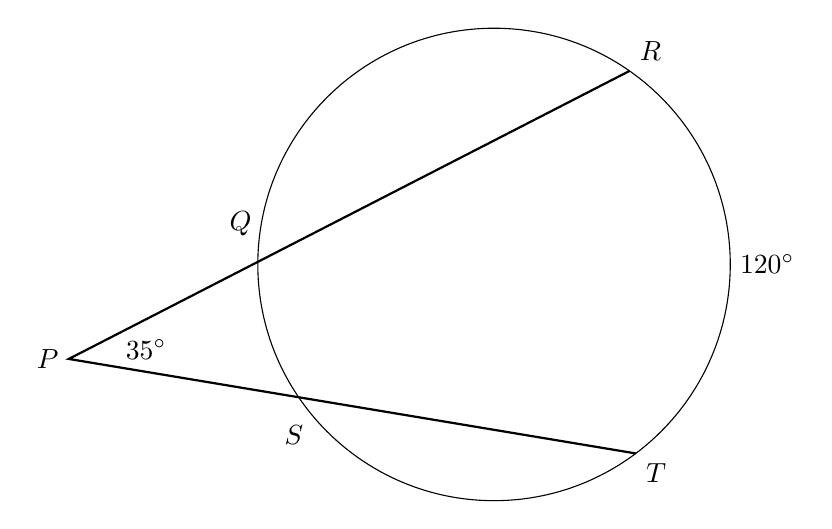
\begin{tikzpicture}[scale=.6]
    \draw (0,0) circle[radius=5];
    \draw [thick]
    (3,-4) node[below right]{$T$}--
    (-9,-2) node[left]{$P$}--
    (55:5) node[above right]{$R$};
    \draw (220:5) node[below left]{$S$};
    \draw (170:5) node[left] {$Q$};
    \draw (0:5) node[right] {$120^\circ$};
    \draw (-8,-1.8) node[right] {$35^\circ$};
  \end{tikzpicture}
\end{center} \vspace{1cm}

\item The secants $\overline{ABC}$ and $\overline{ADE}$ intersect the circle $O$, as shown in the diagram. \\Given $m \wideparen{BD}=28^\circ$ and $m \wideparen{CE}=136^\circ$.
\begin{enumerate}
  \begin{multicols}{2}
    \item Find the $m\angle CDE$.
    \item Find the $m\angle BCD$.
  \end{multicols}  \vspace{1.5cm}
\item Find the $m\angle A$. \vspace{0.5cm}
\end{enumerate}
\begin{center}
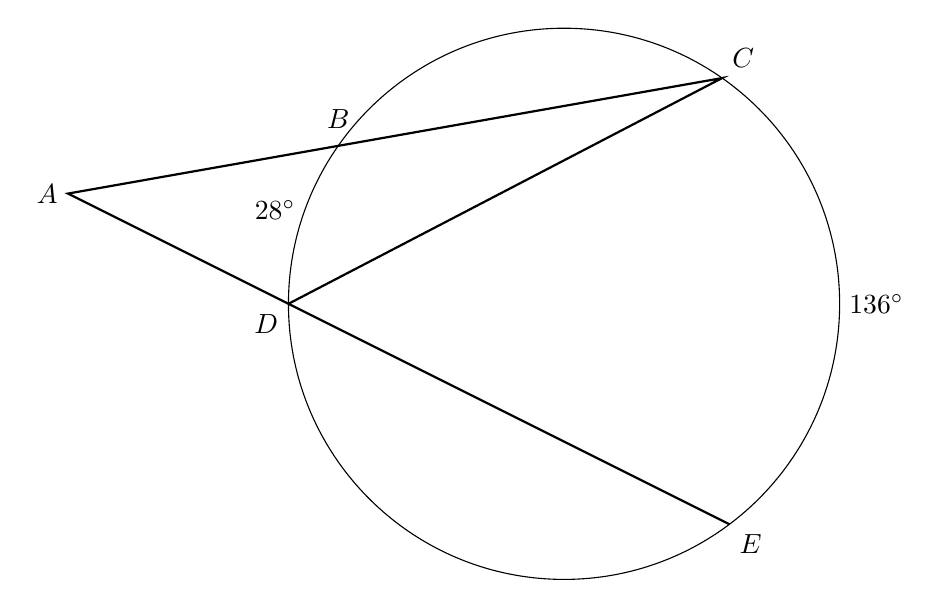
\begin{tikzpicture}[scale=.7]
  \draw (0,0) circle[radius=5];
  \draw [thick]
  (3,-4) node[below right] {$E$}--
  (-5,0) node[below left] {$D$}--
  (-9,2) node[left] {$A$}--
  (55:5) node[above right] {$C$}--
  (-5,0);
  \draw (138:5) node[left] {$B$};
  \draw (0:5) node[right] {$136^\circ$};
  \draw (160:5) node[left] {$28^\circ$};
\end{tikzpicture}
\end{center}

\newpage
\item Write down the center and radius of each circle.
\begin{enumerate}
\begin{multicols}{2}
\item   $(x-4)^2+(y-3)^2=9$ \vspace{2.5cm}
\item   $(x+5)^2+(y-2)^2=4^2$
\item   $x^2+y^2=4$ \vspace{2.5cm}
\item   $(x+7)^2+(y-2)^2=9^2$
\end{multicols}
\end{enumerate}


\item Write down the center and radius of each circle.
\begin{enumerate}
\begin{multicols}{2}
\item   $(x+1)^2+(y-3)^2=49$ \vspace{2.cm}
\item   $(x+4)^2+(y+2)^2=5^2$
\item   $x^2+y^2=20$ \vspace{2.cm}
\item   $(x+1)^2+(y-2)^2=121$
\end{multicols}
\end{enumerate}

\item In right triangle $ABC$ shown below, point $D$ is on $\overline{AB}$ and point $E$ is on $\overline{BC}$ such that $\overline{AC} \parallel \overline{DE}$. Given $BD=10$, $BC=12$, and $EC=4$.
  \begin{center}
  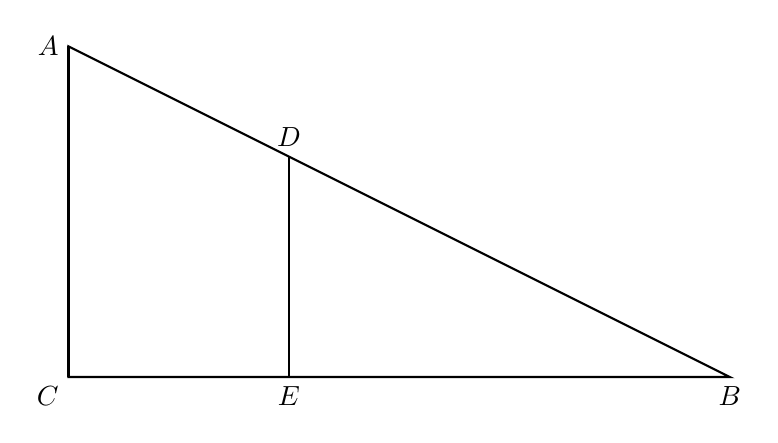
\begin{tikzpicture}[scale=0.7]
    \coordinate [label=left:$A$](A) at (-12,6);
    \coordinate [label=below:$B$](B) at (0, 0);
    \coordinate [label=below left:$C$](C) at (-12,0);
    \coordinate [label=above:$D$](D) at (-8, 4);
    \coordinate [label=below:$E$](E) at (-8,0);
    \draw [thick] (A)--(B)--(C)--cycle;
    \draw [thick] (A)--(C);
    \draw [thick] (D)--(E);
  \end{tikzpicture}
  \end{center}
  \begin{enumerate}
    \item Find the length of $\overline{BE}$. \vspace{0.5cm}
    \item Find the scale factor, $k$, dilating $\triangle DBE \rightarrow \triangle ABC$, centered at $B$. \vspace{1.5cm}
    \item Find the area of $\triangle ABC$. \vspace{2.5cm}
    \item Find the area of $\triangle DEB$. \vspace{2.5cm}
    \item Find the ratio of the areas of the two triangles. \vspace{2.5cm}
  \end{enumerate}

\end{enumerate}
\end{document}
  